\chapter{The LHC and CMS}

The Standard Model provides a precise description of the elementary particles we have known.
But there remains fundamental questions to be answered.
Is there a Higgs boson that provides the mechanism for particles to be massive?
Are there more than one type of Higgs bosons?
Is supersymmetry a real?
What are dark matter and dark energy?
Why is there far more matter than antimatter in the observed universe?
Are there phenomena in particle physics that cannot be explained by the existing theories?

A good way to study these questions at the same time is via high energy hadron collisions.
The Large Hadron Collider is the most powerful hadron collider that human have built for this purpose,
and the Compact Muon Solenoid (CMS) experiment is one of the experiments at the LHC that study the outcome of the collisions. 
An overview of the LHC is given in Section~\ref{sec:lhc}, and the CMS detector is described in Section~\ref{sec:cms}.

\section{The Large Hadron Collider}\label{sec:lhc}

The Large Hadron Collider (LHC)~\cite{Evans_2008} at CERN near Geneva Switzerland is the world's largest and most powerful machine for particle physics research.
It is a double-ring superconducting hadron accelerator and collider installed in a 26.7 \km circular tunnel inherited from its predecessor, the Large Electron-Positron Collider (LEP).
The LHC tunnel lies in the rock stratum between 45 \meter and 170 \meter underground, 
and spans across the French-Swiss border from the bank of the Geneva Lake to the base of the Jura mountain.   
Figure~\ref{fig:lhc_landscape} shows the geographical location of the LHC. 
Two series of hadron bunches rotate in opposite directions in the main LHC ring and collide at four interaction points, 
each hosting a major LHC experiments: Point 1 for ATLAS, Point 2 for ALICE, Point 5 for CMS, and Point 8 for LHCb.

\begin{figure*}[!htb]
    \centering
    \captionsetup{justification=justified}
    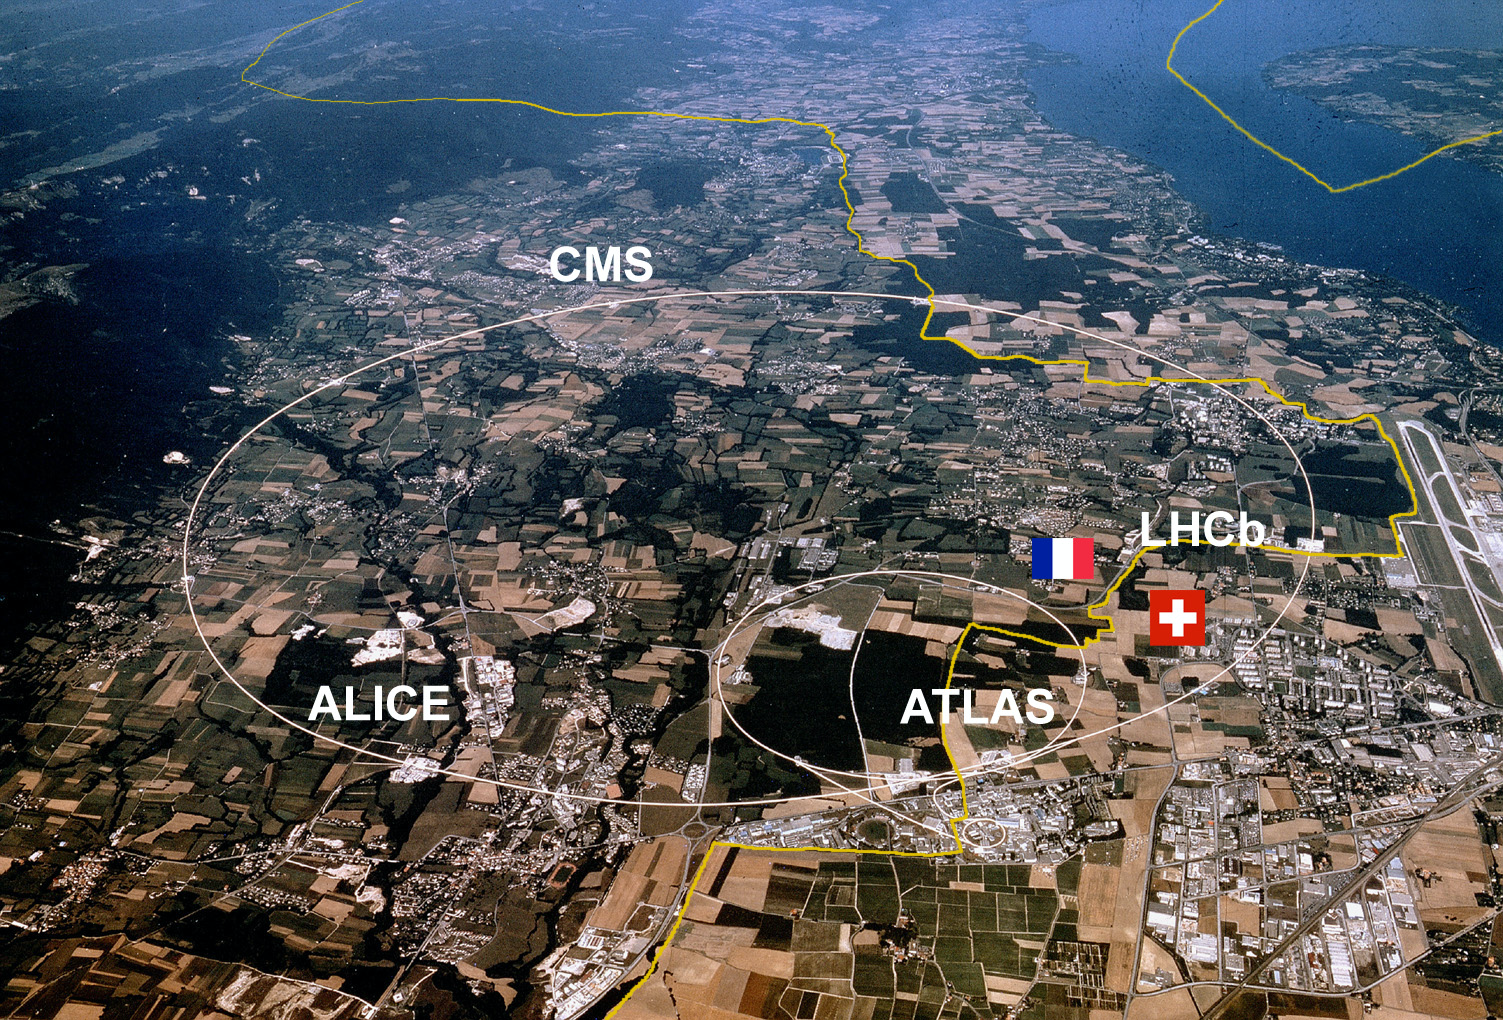
\includegraphics[width=0.95\textwidth]{pics/LHC_CMS/LHC_landscape.png}
    \caption{Photo taken from ... (original source unknown). 
             An aerial view of the LHC landscape. The French-Swiss border is indicated by the yellow line and the LHC tunnels are outlined in white.
             The triangular building complex just below ATLAS in the picture is the main campus of CERN.}
    \label{fig:lhc_landscape}
\end{figure*}

The LHC tunnel consists eight arc and eight straight sections.
The arcs make the majority of the LHC circumference, accommodating thousands of the magnet units to bend and tighten the particles' trajectory.
The straight sections are approximately 528 \meter long each, serving as insertions for experiments or utility. 
The arcs and straight sections are grouped into eight octants, each covering a straight section and two halves of its neighboring arcs,
whose geometrical layout is shown in Figure~\ref{fig:lhc_scheme}. 

\begin{figure*}[!htb]
    \centering
    \captionsetup{justification=justified}
    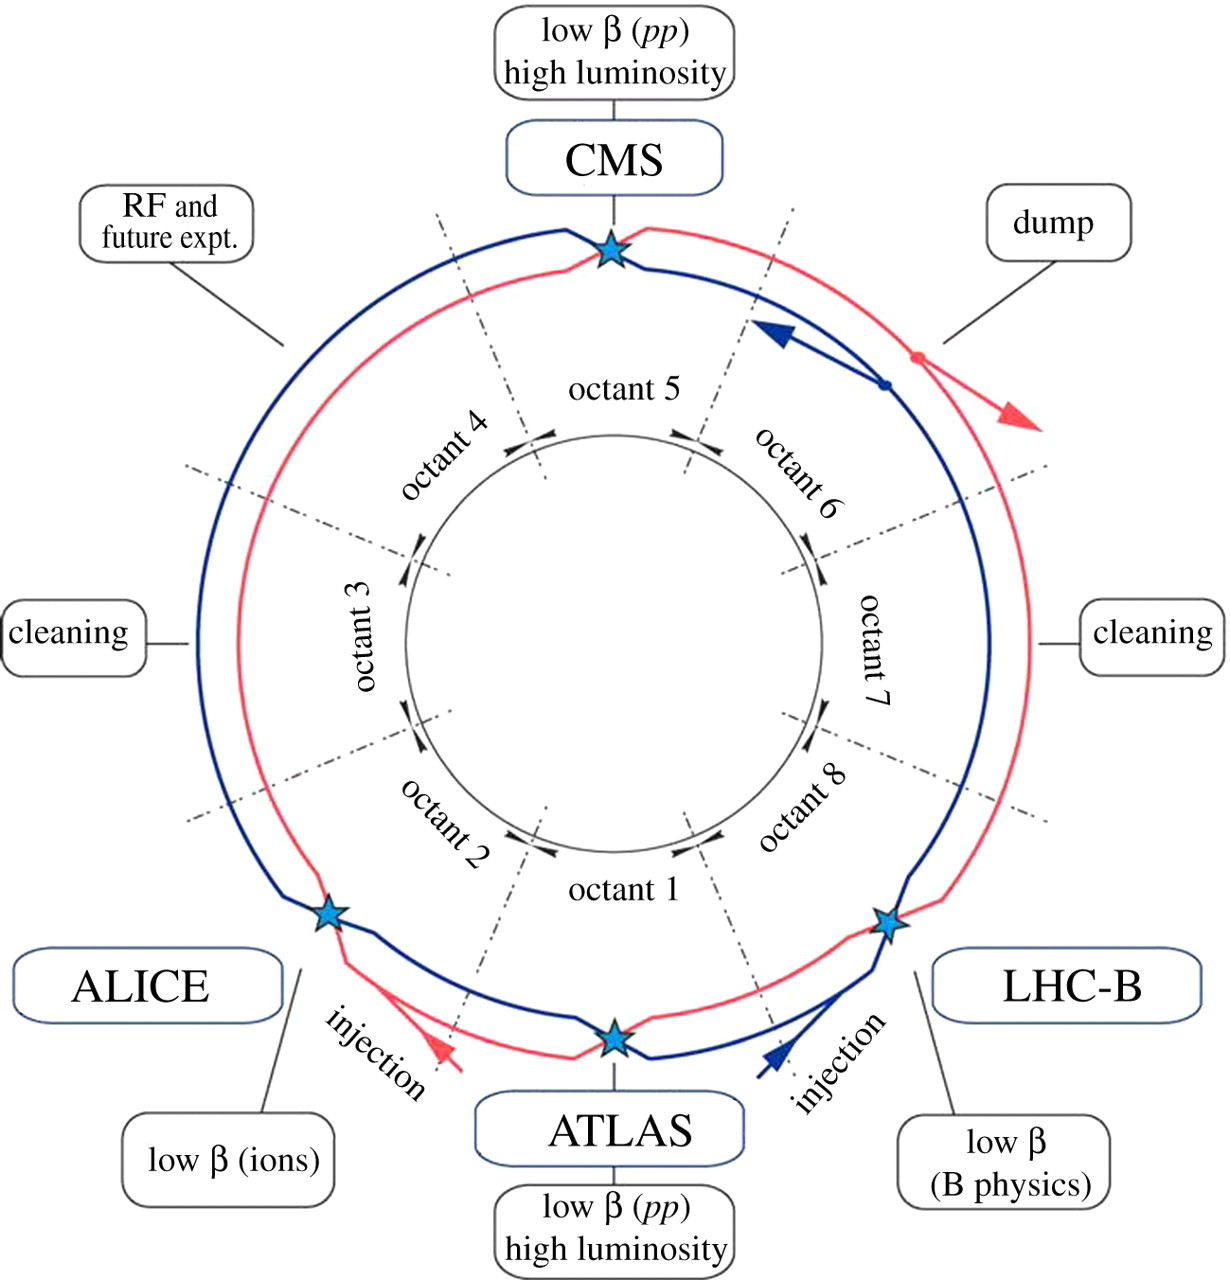
\includegraphics[width=0.85\textwidth]{pics/LHC_CMS/LHC_scheme.jpg}
    \caption{Plot taken from Ref.~\cite{Evans_2008}. 
             The schematic layout of the LHC. Each octant contains a insertion point.
             Points 1, 2, 5, and 8 are the locations of collision experiments. Points 3 and 7 are for beam collimation. 
             Hadrons are injected at Points 1 and 8, accelerated at Point 4, and eventually discarded at Point 6.}
    \label{fig:lhc_scheme}
\end{figure*}

\begin{figure*}[!htb]
    \centering
    \captionsetup{justification=centering}
    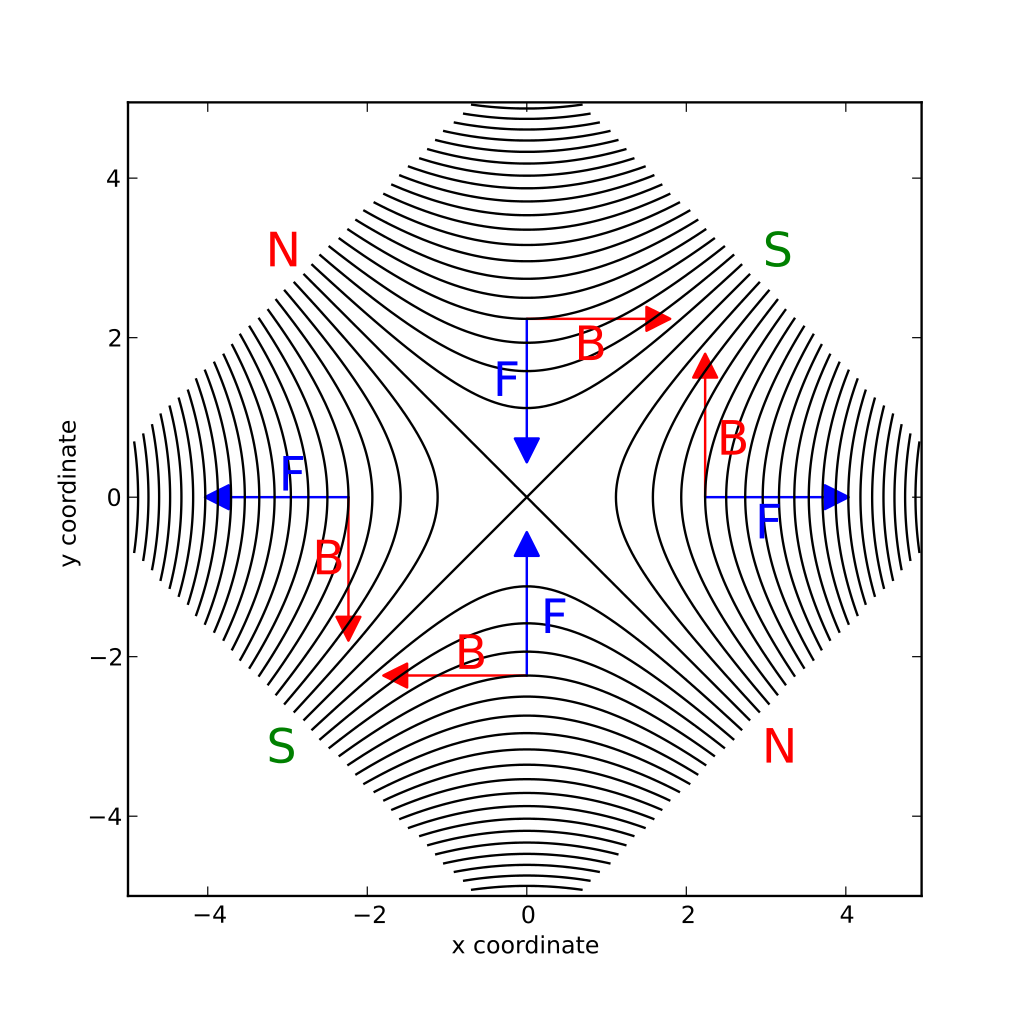
\includegraphics[width=0.85\textwidth]{pics/LHC_CMS/quadrupole_field.png}
    \caption{Plot taken from Ref.~\cite{quadrupole_wiki}. 
             Magnetic field of an ideal quadrupole.}
    \label{fig:quad_field}
\end{figure*}

Strong magnets are what guide the high energy hadrons to circulate and collide in the LHC. 
The LHC magnet system is based on Nb-Ti cables, cooled by superfluid helium to a temperature of 1.9 K,
where the cables stay superconductive and generate a magnetic field up to their critical field strength.
The maximum operable magnetic field of the LHC magnets is 8.33 T, which corresponds to a proton beam energy of 7 \TeV,
or a heavy ion beam energy of 2.76 \TeV per nucleon.

The LHC magnet system consists 1232 main dipole magnets, about 450 quadrupole magnets,
a few thousands multipole corrector magnets, and several types of specialized magnets at the eight insertion points.
The dipoles 
bend the beams so they circulate in the LHC tunnel.
Since the both beams are positively charged but travel in opposite directions,
the magnetic fields for the two beams need to be opposite as well.
Given the space limitation in the tunnel and the need to keep the budget down, a "twin-bore" design is adopted, 
in which the two beam pipes and two sets of magnet coils are installed next to each other in the same piece of mechanic housing, called the cold mass.
The cold mass is a cylindrical solid iron structure bored at its center and surrounded by a superfluid helium vessel.
Each cold mass has a length of about 15 \meter, a diameter of about 570 \mm, and a mass of about 27.5 t.
It provides a stable 1.9 K environment for the magnet coils, and in the meantime serves as their magnetic yoke.
The dipoles of LHC are manufactured identically up to a high precision.
The relative variation in the magnetic field strength and the field inhomogeneity must not exceed $10^{-4}$,
The quadrupoles 
provide gradient fields (shown in Figure~\ref{fig:quad_field}) that squeeze the beam in one direction and disperse it in the other.
A few quadrupoles in series, with certain field geometry, can focus or defocus the beams.
They keep the beams from dispersing in the beam pipes, focus the beams to high intensity before collisions, and defocus them after collisions.
Quadrupoles are also in stationed in twin-bored cold masses, each about 3.1 \meter long.
Several types 
of small-scale multipole correctors are installed as components of the main dipoles and quadrupoles, 
which help to fine-tune the beam parameters. 
The insertion magnets 
serves various purposes: to adjust the beam parameters to the needs of each dedicated experiment, 
or to abruptly change the direction of the beam for injection or abortion.
Most insertion magnets are based on Nb-Ti superconductors, 
while some, in radiation areas, are built of normal conducting material.
The electric currents in these various magnets range from 60 A (for small correctors) to 12 kA (for main dipoles and quadrupoles),
while the total energy stored in the magnets is about 10 GJ during full operations of the LHC.

\begin{figure*}[!htb]
    \centering
    \captionsetup{justification=justified}
    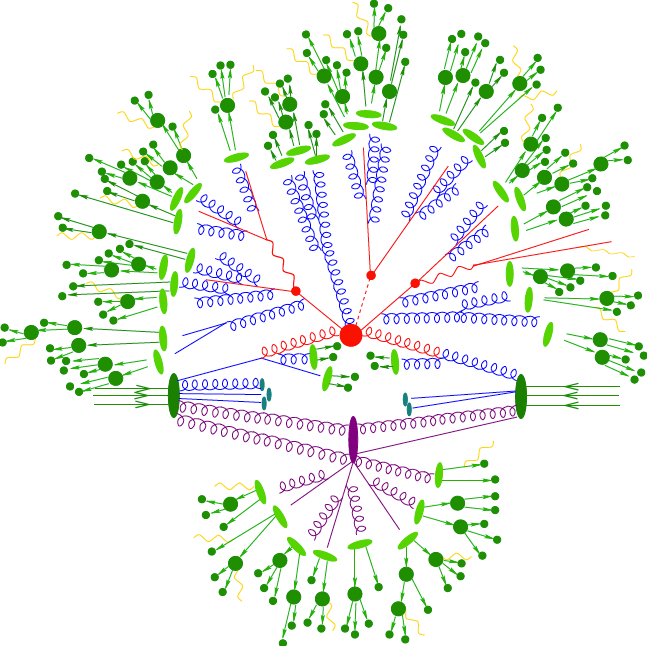
\includegraphics[width=0.70\textwidth]{pics/LHC_CMS/sherpa_sim.png}
    \caption{Plot taken from Ref.~\cite{Gleisberg_2009}. 
             An illustration of the interactions in a $pp$ collision.
             The primary interaction in this example is the Higgs boson production in association with a top quark pair, 
             whose Feynman diagram is shown in ~\ref{fig:main_higgs_modes}.}
    \label{fig:sherpa_pp}
\end{figure*}

Proton-proton ($pp$) collisions at the LHC initiate a diverse range of processes.
Quarks and gluons, together called partons, in protons can initiate QCD processes, 
in which a cascade of quarks and gluons are produced, which in turn hadronize and form various hadrons at high multiplicity.
Quarks also participate in the electroweak interaction, producing gauge bosons, which may decay to leptons.
The Higgs boson can be from quarks and gauge bosons.
In $pp$ collisions, partons carry a fraction of the proton energy, 
following a broad spectrum called the parton distribution function (PDF).
As a result, the energy of each interaction can vary in a broad range.
Furthermore, protons, compared to antiprotons and positrons, are easy to obtain and accelerate,
allowing for collisions at high energy and high luminosity.
Overall, $pp$ collisions can generate all physics processes in a wide energy spectrum with a large statistical sample size, 
making a ideal tool to perform generic searches for expected and unexpected physics processes. 

Figure~\ref{fig:sherpa_pp} demonstrates an example of the interactions initiated in a hard $pp$ scatter instance.
The primary interaction in this example is the production of the Higgs boson associated with a top quark pair (\ttH),
in which the loopy red lines present the incoming gluons, the big red blob is the vertex of the primary interaction,
and the small red blobs are the decay vertices of the Higgs boson and the top (anti-top) quarks.
Additional QCD radiations are indicated by the loopy blue lines, which undergo hadronization (light green blobs) and form hadrons (dark green blobs). 
The hard interaction in this example is accompanied with a softer secondary interaction (purple blob), 
which produce a bunch of hadrons through QCD processes.
Finally, photons (curvy yellow lines) can be emitted from the final state hadrons and leptons.

At the LHC, multiple $pp$ collisions are expected in each proton bunch crossing, known as pileup.
In most cases, all of these simultaneous interactions are QCD interactions, 
while occasionally one of the collisions is a hard scatter that leads to processes interesting to physicists.
In those occasions, the collision containing the hard scatter is considered as the primary interaction, 
and the other collisions are called pileup interaction.
Within the primary interaction, the process of interest, for example the \ttH process in Figure~\ref{fig:sherpa_pp},
is called the prompt interaction, while the other QCD-induced byproducts are called the underlying event.

\section{The Compact Muon Solenoid experiment}\label{sec:cms}


The Compact Muon Solenoid (CMS)~\cite{Collaboration_2008} is a general purpose detector operating at one of the collision sites of the LHC.
It is named after its large-bore superconducting solenoid magnet, 
which provides a 4 T field at its core and enables precise measurements of the various collision products.
The CMS detector has an overall length of 28.7 \meter, a diameter of 15.0 \meter and a weight of 14000 t.
A cutaway diagram of CMS is shown in Figure~\ref{fig:cms_detector}.
It consist, from inside to outside, of a silicon-based tracking system (blue slices in the figure), 
a lead tungstate crystal electromagnetic calorimeter (ECAL) (cyan blocks),
a brass-scintillator hadron calorimeter (HCAL) (yellow blocks),
a superconducting solenoid (white blocks), 
and an iron return yoke (red blocks) interleaved with a multi-layer muon detector (white panels).

\begin{figure*}[!htb]
    \centering
    \captionsetup{justification=justified}
    \includegraphics[width=0.95\textwidth]{pics/LHC_CMS/cms_phase1.pdf}
    \caption{Plot taken from Ref.~\cite{Sakuma:2665537}. 
             A cutaway diagram of the CMS detector. 
             The design is specified to a design stage called the Phase-1 detector upgrade~\cite{arXiv:2012.14304, Mans:1481837,Tapper:1556311}.}
    \label{fig:cms_detector}
\end{figure*}

CMS adopts a spherical coordinates convention: the origin is positioned at the geometrical center of CMS expected for collisions to happen;
the $z$ axis is along the beam pipe with its positive direction pointing toward the Jura mountain;
the $\phi = 0$ direction (or the $x$ axis of the Cartesian coordinates) points horizontally toward ATLAS at the opposite side of the LHC tunnel;
this leaves the $y$ axis of the Cartesian coordinates pointing upward to the sky.
In addition, the polar angle $\theta$ is in most cases replaced by a variable called pseudorapidity $\eta$, 
defined as $\eta = -\text{ln}[\text{tan}(\frac{\theta}{2})]$.
The pseudorapidity is a good approximation of the longitudinal rapidity $y_{L}$ of particles in the CMS frame in the limit of $|\textbf{p}| \gg m$.
The CMS coordinates, along with the $\eta - \theta$ correspondence, are shown in Figure~\ref{fig:cms_longitudinal}.

\begin{figure*}[!htb]
    \centering
    \captionsetup{justification=justified}
    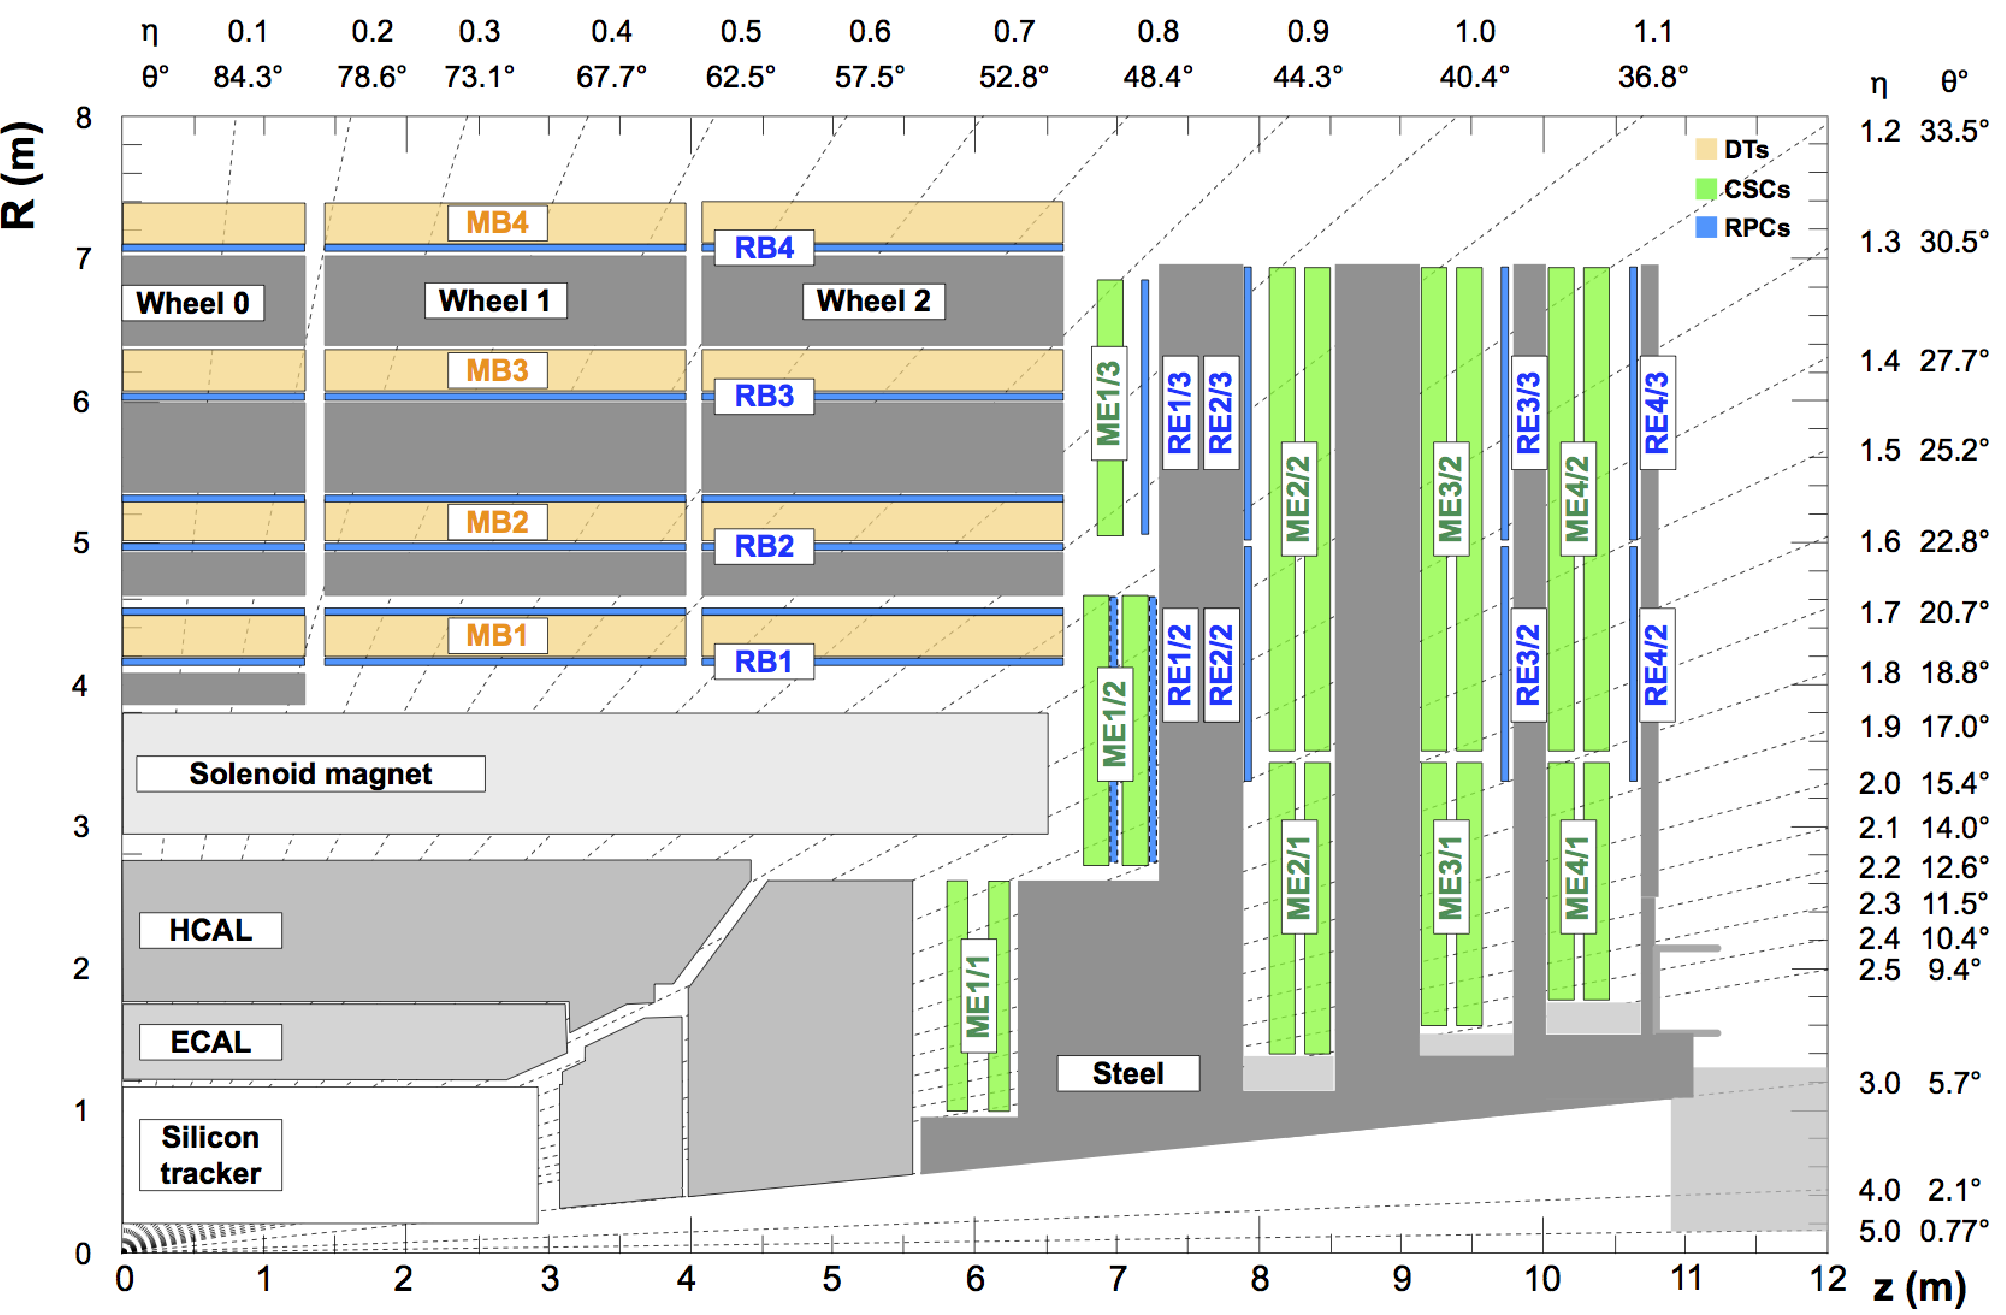
\includegraphics[width=0.95\textwidth]{pics/LHC_CMS/CMS_longitudinal.png}
    \caption{Plot taken from Ref.~\cite{Sirunyan_2018}. 
             A longitudinal section view of the CMS detector, gridded with the CMS coordinates.}
    \label{fig:cms_longitudinal}
\end{figure*}


The solenoid magnet of CMS is based on the same material as the LHC magnets, operating also at 1.9 K.
During its full operation, the superconducting coil carries an electric current of 18500 A and stores an energy of 2.6 GJ.
It generates a homogeneous 4 T field inside its bore of 6-\meter diameter and 12.5-\meter length,
providing the functioning environment for the detector components installed inside of it.
The superconducting coil is enclosed by its iron yoke, which is the heaviest part of the CMS detector, 
weighing about 12000~t, almost twice as much iron in the Eiffel Tower.
The iron yoke guides the magnetic field outside of the coil, and in the meantime serves as the supporting frame for all other CMS detector components.
Figure~\ref{fig:cms_field} shows the operating magnetic field of CMS.

\begin{figure*}[!htb]
    \centering
    \captionsetup{justification=justified}
    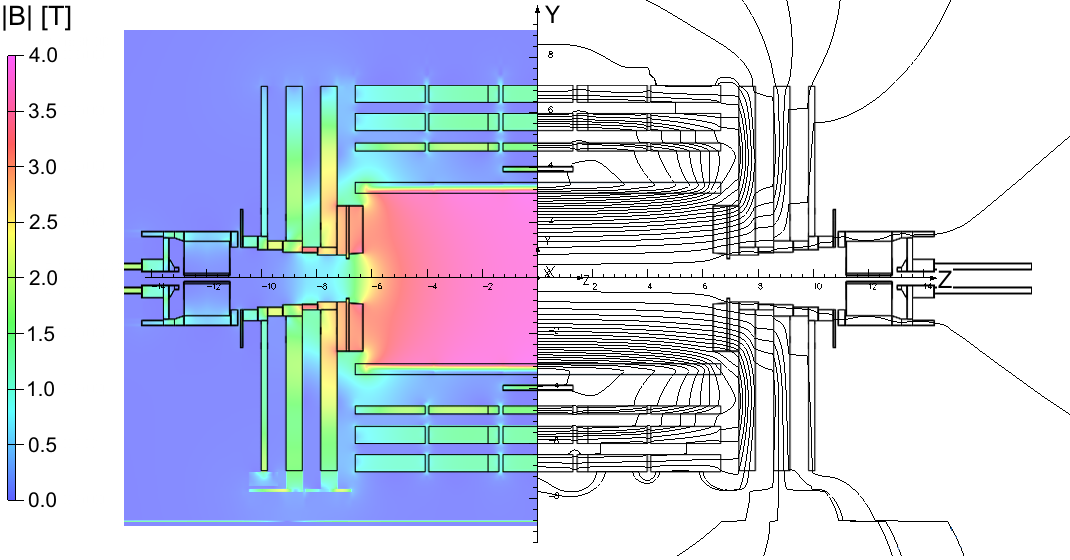
\includegraphics[width=0.95\textwidth]{pics/LHC_CMS/CMS_field.png}
    \caption{Plot taken from Ref.~\cite{Collaboration_2010}. 
             The magnetic field in CMS displayed in a longitudinal section, operating with a central field strength of 3.8 T.
             The field value $|B|$ is shown on the left and the field lines are shown on the right.}
    \label{fig:cms_field}
\end{figure*}


The CMS inner tracker is designed to provide a precise and efficient measurement of the trajectories of charged particles emerging from the LHC collisions.
It is laid out in a cylindrical volume of 5.8-\meter length and 2.5-\meter diameter surrounding the beam pipe, shown in Figure~\ref{fig:cms_tracker}.
It is composed of a pixel detector with four barrel layers at radii of 2.9~\cm, 6.8~\cm, 10.9~\cm, and 16.0~\cm~\cite{phase1_tracker},
and a silicon strip detector with 4 + 6 barrel layers extending to a radius of 1.1~\meter~\cite{Collaboration_2008}.
Each system is completed by endcaps which consist of three disks in the pixel detector and 3 + 9 disks in the strip detector.
The CMS tracker has about 124 million pixels channels and about 9.3 million strip channels in total,
and provides its full tracking ability up to a pseudorapidity range of $|\eta| < $2.5.

\begin{figure*}[!htb]
    \centering
    \captionsetup{justification=justified}
    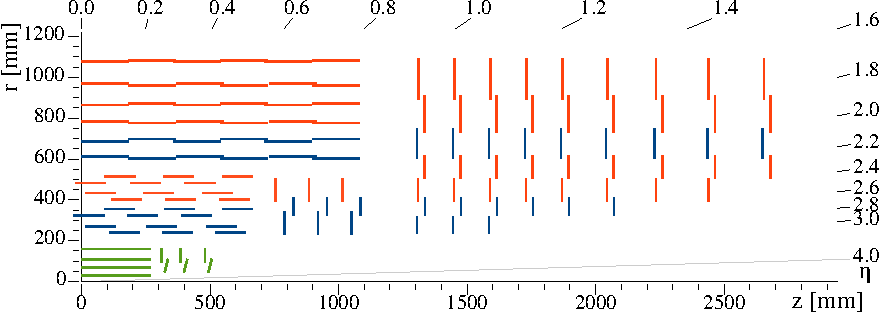
\includegraphics[width=0.95\textwidth]{pics/LHC_CMS/Phase1_Tracker.pdf}
    \caption{Plot taken from Ref.~\cite{phase1_tracker}. 
             Sketch of one quarter of the Phase-1 CMS tracking system in r-z view.
             The pixel detectors are shown in green, 
             while single-sided and double-sided strip modules are depicted as red and blue segments, respectively.}
    \label{fig:cms_tracker}
\end{figure*}

In the pixel detector, the standard pixel size is 100 $\times$ 150 $\mum^{2}$ in $r\phi \times z$ plane, with a thickness of 285~\mum.
At the nominal LHC luminosity, about 1000 charged particles are produced in each bunch crossing, 
corresponding to a hit occupancy of the order $10^{-4}$ per pixel per bunch crossing.

At its operation, a charged particle usually generate signals in a few neighboring pixels, known as the charge-sharing.
The pixel system reads with analog pulse height read-out, which enables an interpolation between the neighboring pixels
and achieves a spatial resolution in the range of 15-20~\mum.

The strip detector is made up of two subsystems in two regions, the inner region ($20 \cm < r < 55 \cm$) 
and the out region ($55 \cm < r < 110 \cm$), both composed of silicon micro-strip detectors. 
A typical micro-strip cell in the inner region has a thickness of 320 \mum and size of 10~\cm~$\times$~80~\mum,
leading to an occupancy of of up to 2-3\% per strip per LHC bunch crossing.
Micro-strip cells in the outer region, given the larger radii and reduced particle density, are larger in size:
500 \mum in thickness and up to about $25 \cm \times 180 \mum$ in size,
and corresponding to an occupancy of about 1\%.
The spatial resolution of the strip cells, after the interpolation of charge-sharing, 
ranges from 23-35~\mum in the inner barrel layers, and from 35-53~\mum in the outer barrel layers.  

All strip cells are placed parallel to the beam pipe in the barrel, and along the radial direction in the endcaps.
To provide a measurement of the coordinate along the strip length (z in the barrel and r in the endcaps),
some layers of the strip detector are constructed with a double-strip design, 
in which a second micro-strip detector module is mounted back-to-back to each original strip module with a stereo angle of 100 mrad. 
This measurement achieves a resolution of 230~\mum in the inner barrel and 530~\mum in the outer barrel, 
while the resolution varies in the endcap disks depending on the hit location.

The whole tracking system, consisting of the numerous silicon sensors and their read-out system,
consumes about 60~kW of electric power, which in turn is dissipated as heat in the tracker volume.
A cooling system is built to maintain its operation temperature of -10~${}^{\circ}$C, 
in which the pixel layers are cooled with aluminum conducting tubes, 
and the strip layers are cooled with a continuous flow of $\text{C}_{6}\text{F}_{14}$ liquid.




%\section{Trigger system in CMS}

%\section{Level-1 Trigger}